\documentclass[10pt,twocolumn,letterpaper]{article}

\usepackage{cvpr}
\usepackage{times}
\usepackage{epsfig}
\usepackage{graphicx}
\usepackage{amsmath}
\usepackage{amssymb}
\usepackage{mathtools}
\usepackage{multicol}

\DeclarePairedDelimiter\abs{\lvert}{\rvert}%

% Include other packages here, before hyperref.

% If you comment hyperref and then uncomment it, you should delete
% egpaper.aux before re-running latex.  (Or just hit 'q' on the first latex
% run, let it finish, and you should be clear).
\usepackage[breaklinks=true,bookmarks=false]{hyperref}

\cvprfinalcopy % *** Uncomment this line for the final submission

\def\cvprPaperID{****} % *** Enter the  Paper ID here
\def\httilde{\mbox{\tt\raisebox{-.5ex}{\symbol{126}}}}

% Pages are numbered in submission mode, and unnumbered in camera-ready
\setcounter{page}{1}
\begin{document}

%%%%%%%%% TITLE
\title{EE3-23: Coursework for Introduction to Machine Learning}

\author{Douglas Brion\\
Imperial College London\\
CID: 01052925\\
{\tt\small db1415@ic.ac.uk}
}

\maketitle
%\thispagestyle{empty}


%%%%%%%%% BODY TEXT
\section{Introduction}

This report examines different approaches to predicting wine quality using the Wine Quality~\cite{WineQuality} dataset. This is a large dataset containing 4898 samples of white wines and 1599 red. Throughout this report wine quality is examined using regression, the standard approach when modelling continuous data, attempting to predict the quality of a wine from various input parameters. Multiple learning methods are implemented, discussed and compared in order to obtain a predictor with the smallest test error possible.

All code for this report was written in Python using the libraries Pandas~\cite{mckinneypandas} for importing and manipulating data and Tensorflow~\cite{tensorflow2015-whitepaper} for creating and training models to predict the data.

The objective of this report is to identify the predictor with the best regression performance.

%-------------------------------------------------------------------------
\section{Data Preparation}
As red and white wine have different tastes, it was decided to learn on them separately as they differ in chemical composition. The objective in this report is to establish how well the quality of each wine can be predicted using the datasets.

It should be noted that this data is likely to be unreliable and noisy for quality was measured with a human sense, taste, a very personal metric which can range widely from person to person.

The data was normalised with respect to it's mean and to a standard deviation of one. Outliers over a threshold of for each attribute were removed to reduce noise in the dataset for training. Tab \ref{tab:normalised} shows the normalised physiochemical attributes for the datasets with outliers removed. 

\begin{figure}[h]
	\begin{center}
		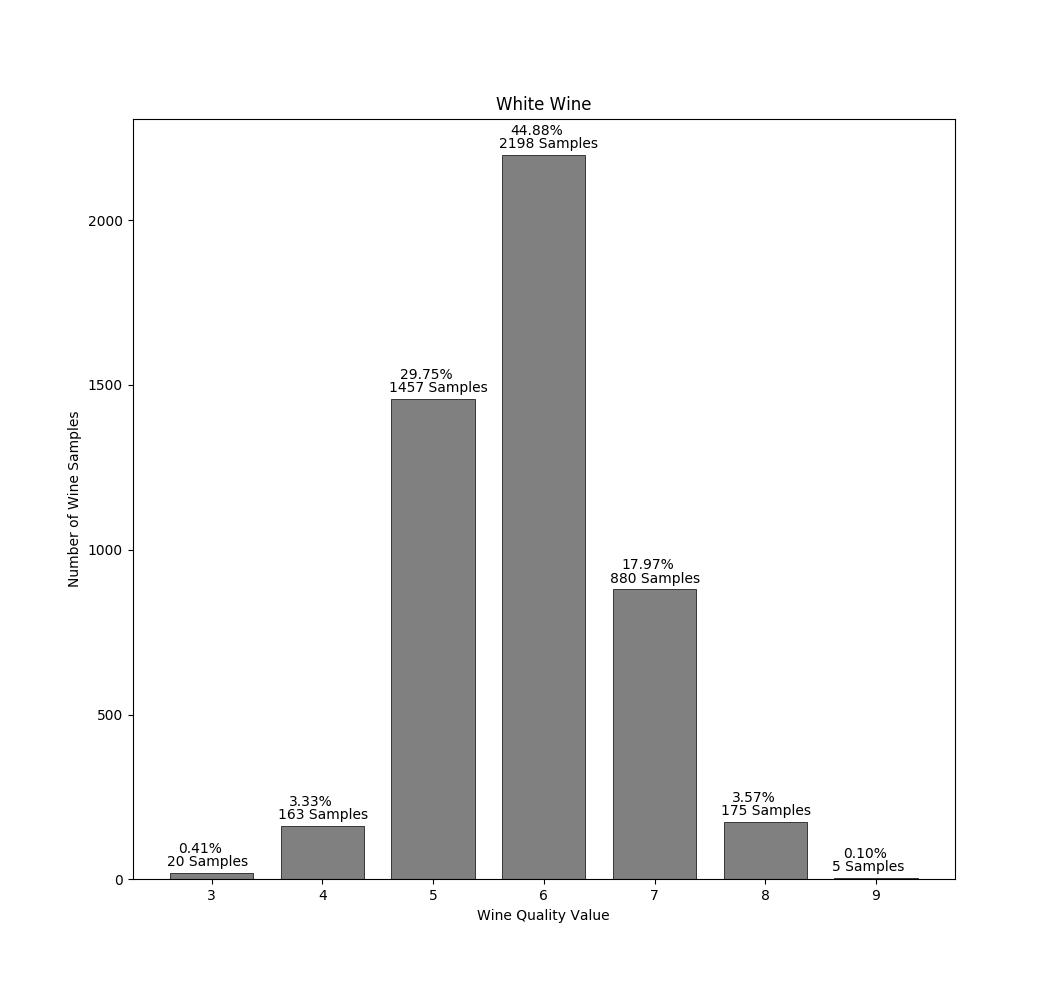
\includegraphics[width=0.8\linewidth]{img/white_samples.png}
	\end{center}
	\caption{The histogram for white wine qualities.}
	\label{fig:histwhite}
\end{figure}

\begin{figure}[h]
	\begin{center}
		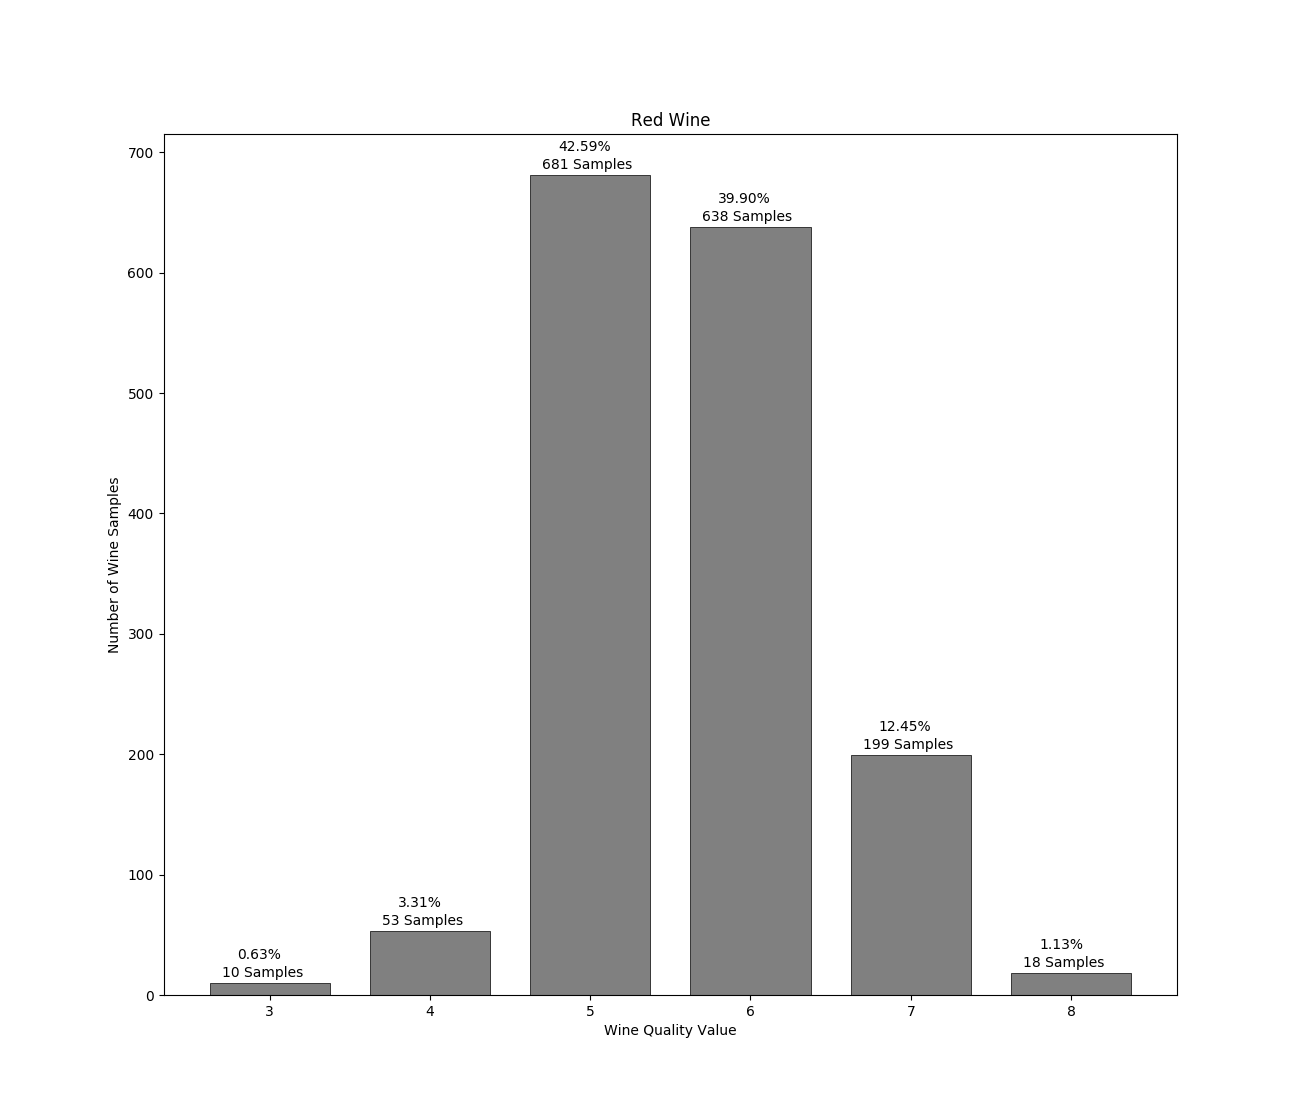
\includegraphics[width=0.8\linewidth]{img/red_samples.png}
	\end{center}
	\caption{The histogram for red wine qualities.}
	\label{fig:histred}
\end{figure}

\begin{table*}
	\begin{center}
		\begin{tabular}{|l|cc|cc|cc|cc|}
			\hline
			Attributes 			& Mean 	& 		& Std 	& 		& Min 	& 		& Max 	&		\\
								& White & Red 	& White & Red 	& White & Red 	& White & Red \\
			\hline
			fixed acidity 		& -0.003 & 0.000 & 0.989 & 1.000& -3.62 &-2.137 & 4.557 & 4.355 \\
			volatile acidity 	& -0.012 & -0.004 & 0.961 &0.989 & -1.967 &-2.278& 4.979 & 4.481\\
			citric acid 		& -0.010 & 0.000 & 0.963 & 1.000&-2.762 &-1.391& 4.758 & 3.744\\
			residual sugar 		& -0.002 & -0.053 & 0.986 & 0.764&-1.142 &-1.163& 4.971 & 4.584\\
			chlorides 			& -0.078 & -0.096 & 0.662 &0.552 &1.683 &-1.604& 4.954 & 3.880\\
			free sulfur dioxide & -0.010 & -0.003 & 0.956 & 0.991&-1.959 &-1.423& 4.892 & 4.985\\
			total sulfur dioxide & -0.003 & -0.009 & 0.992 & 0.967&-3.044 &-1.231& 4.839 & 3.604\\
			density 			& -0.005 & 0.000 & 0.971 & 1.000&-2.313 &-3.539& 2.984 & 3.680\\
			pH 					& 0.000 & 0.000 & 1.000 & 1.000&3.101 &-3.700& 4.184 & 4.528\\
			sulphates 			& -0.001 & -0.033 & 0.997 & 0.879&-2.365 &-1.936& 4.996 & 4.142\\
			alcohol 			& 0.000 & -0.000 & 1.000 &1.000 &-2.043 &-1.899& 2.995 & 4.202\\ 
			\hline
		\end{tabular}
	\end{center}
	\caption{The white and red wine attribute statistics after removal of outliers and normalisation.}
	\label{tab:normalised}
\end{table*}

The spread in quality for both data sets is not ideal for learning with the histograms Fig \ref{fig:histwhite} and Fig \ref{fig:histred} illustrating the distribution. The quality of the wine is graded on a scale from 0 (really bad) to 10 (extremely good) with the datasets containing six/seven classes (3 to 8/9). The red wine dataset is especially concentrated in the quality values 5 and 6. 

\subsection{Learning approach}

For consistency the performance of each model with varying parameters and training cost functions will be measured using the same error metric, the Huber Loss function. This is a good loss function for this regression problem as it is robust to outliers, for if the difference between the real and predicted value is small it will be squared, if large, the absolute value will be taken.

\begin{equation}
L_H = \begin{cases}
 \frac{1}{2} (y - f(x))^2, & \text{for\ } \abs{y - f(x)} \leq \delta. \\
 \delta \abs{y - f(x)} - \frac{1}{2} \delta^2, & \text{otherwise.}
\end{cases}
\label{eq:huber}
\end{equation}

A robust procedure for estimation was used, \textit{k}-fold cross validation~\cite{CrossValidation}, where data is divided into \textit{k} parts and with one subset tested at a time and remaining data used for training. This methods results in all data being used for both training and testing, however requires a longer computation time.

\section{Baseline Predictors}
Several baseline predictors have been implemented and trained on the data. 

A linear regression program was written in Python using Tensorflow~\cite{tensorflow2015-whitepaper}. This linear model used an iterative method to alter the weights, with multiple loss functions tested. This proved useful as a framework for the more advanced algorithms implemented later on.

For linear regression 2 basic loss functions were implemented first.

\subsection{LASSO loss function}
The LASSO loss function tries to minimise the absolute difference between the predicted and real values. The sum of all the differences for all the samples can be described as follows:

\begin{equation}
L_{LASSO} =  \abs{y - f(x)}
\label{eq:lasso}
\end{equation}

This is a fairly robust loss function which is not that affected by outliers. 

\subsection{Ridge loss function}
The Ridge loss function, least square error, minimises the square difference between the predicted and real values. This value is much larger than that of LASSO loss and therefore is more affected by outliers, however, will optimise the predictor faster.

\begin{equation}
L_{Ridge} =  (y - f(x))^2
\label{eq:ridge}
\end{equation}

Notice how the predictor using the Ridge loss function in \ref{fig:l2loss} minimises the error faster than the LASSO loss in \ref{fig:l1loss}. Additionally, as outliers have been removed in data preparation the Ridge loss is also quite robust.

As the epochs are increased the optimiser is able to reduce the loss until no substantail improvements are made. The learning rate also greatly affects the rate at which the loss is minimised. However, if the learning rate is too high the predictor might not improve in training and may get worse, as can be seen in \ref{fig:break}. (see \textbf{Appendix} to compare LASSO and Ridge)

\begin{figure}[h]
	\begin{center}
		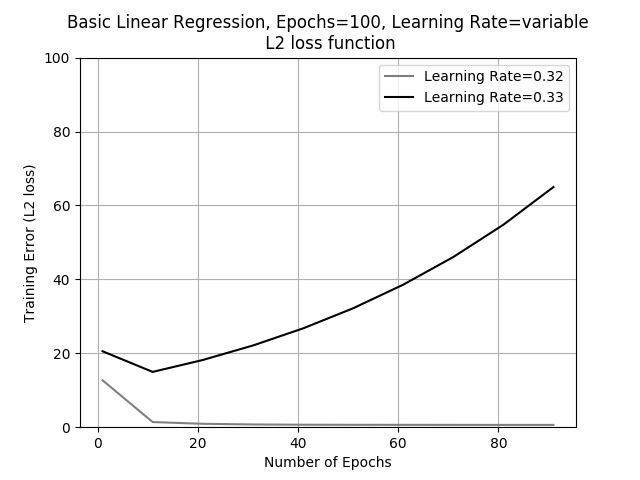
\includegraphics[width=0.8\linewidth]{img/linrbreak.png}
	\end{center}
	\caption{Loss function = Ridge, Epochs = 100, Learning Rate = variable}
	\label{fig:break}
\end{figure}

\subsection{Regularisation}
These relatively simple models can be improved upon by adding regularisation. Regularisation is a technique used to prevent over-fitting the data. Both $L_1$, $L_2$ and Elastic Net regularisation have been implemented, being the sum of the weights and sum of the square weights and combination of the two respectively. The regularisation term is added to the loss function, the terms for $L_1$ and $L_2$ look as follows:

\begin{center}
\noindent\begin{minipage}{.5\linewidth}
	\begin{equation}
	L_1 = \lambda  \abs{w}
	\label{eq:reg1}
	\end{equation}
\end{minipage}%
\begin{minipage}{.5\linewidth}
	\begin{equation}
	L_2 = \lambda  \abs{w}^2
	\label{eq:reg2}
	\end{equation}
\end{minipage}
\end{center}

The elastic net regularisation combines the $L_1$ and $L_2$ penalties of the methods described in Eq \ref{eq:reg1} and Eq \ref{eq:reg2}. A hyper-parameter, $\alpha$ between 1 and 0 controls how much of $L_1$ and $L_2$ penalisation is used.

\begin{equation}
L_{elastic} =  \lambda (\alpha\abs{w} + (1-\alpha)\abs{w}^2)
\label{eq:elastic}
\end{equation}

The computation time for elastic net regularisation is longer than standard LASSO or Ridge due to the additional hyper parameter $\alpha$. 

\section{More Advanced Algorithms}
More advanced algorithms such as Neural Networks can achieve high performance due to their non-linear learning capabilities. However due to this, these complex models are more likely to over-fit, losing the ability to generalise when given new data to test. Linear Support Vector Regression and Neural Networks have multiple hyper-parameters which need to be adjusted in order to find the best predictor.

\subsection{Neural Network}
Neural networks have an advantage over standard linear regression that they can model non-linearities automatically however they are more likely to over-fit the data so observing the out of sample error is especially important.

The neural network implemented as a predictor for this report consisted of 3 layers: input, hidden and output. A single hidden layer was chosen as an increase in hidden layers did not result in a superior predictor performance, although computation time was lengthened.

The number of nodes in the hidden was heuristically chosen as the mean of input and output layers, in this case resulting in 6 hidden nodes.

Whilst being constructed, each layer in the network can be set to a specific activation function such as: TanH, Sigmoid, ReLU, SeLU and Softmax. It was discovered during training that hidden and output ReLU layers resulted in the best out of sample test error this activation function was chosen. 

The neural net used a gradient descent optimiser to minimise the loss function, and either $L_1$, $L_2$ or no regularisation was selected for training. 

\subsection{Support Vector Machine Regression}


The goal for a SVM regression~\cite{Cortes1995} predictor is to find a predication $f(x)$ as with all predictors, however it should have at most $\epsilon$ deviation from the real value $y$ for all the in sample data.

A great advantage SVM methods have over neural networks is that they can guarantee a global over a local minimum. The loss function for SVM regression is as follows:

\begin{equation}
L_{SVR} = \begin{cases}
0, & \text{if\ } \abs{y - f(x)} \leq \epsilon \\
\abs{y - f(x)} - \epsilon, & \text{otherwise.} \\
\end{cases}
\label{eq:svr}
\end{equation}

For the tests run and presented in this report the value of $\epsilon$ was set to $0.5$.

\section{Results}
In order to evaluate the possible models to find the best predictor, 10-fold cross validation was run on each model ($90\%$ training, $10\%$ testing). Graphs of the results will illustrate the average error over cross validation of the predictor across the epochs with the final error for that models loss function shown as 'final error' in the legend. 
The final model after learning is then tested using Huber Loss \ref{eq:huber} also shown in the legend. This is used to compare the various models against each other after training.

\subsection{Linear Regression}
Results were gathered for many combinations of linear regression parameters and cost functions, the results for the best of each for white and red wine is shown below in Tab \ref{tab:whiteresults} and Tab \ref{tab:redresults}.

\begin{table}[h]
	\begin{center}
		\scalebox{0.7}{
		\begin{tabular}{l|l|l|l|l|}
			\cline{2-5}
			& LASSO                                                                             & Ridge                                                                             & SVR                                                                                & Huber                                                                              \\ \hline
			\multicolumn{1}{|l|}{No Reg}          & 0.264                                                                             & 0.260                                                                             & 0.271                                                                              & 0.256                                                                              \\ \hline
			\multicolumn{1}{|l|}{L1 Reg}          & \begin{tabular}[c]{@{}l@{}}$\lambda = 0.0001$\\ 0.261\end{tabular}                & \begin{tabular}[c]{@{}l@{}}$\lambda = 0.001$\\ 0.268\end{tabular}                 & \begin{tabular}[c]{@{}l@{}}$\lambda = 0.001$\\ 0.267\end{tabular}                  & \begin{tabular}[c]{@{}l@{}}$\lambda = 0.01$\\ 0.265\end{tabular}                   \\ \hline
			\multicolumn{1}{|l|}{L2 Reg}          & \begin{tabular}[c]{@{}l@{}}$\lambda = 0.0001$\\ 0.265\end{tabular}                & \begin{tabular}[c]{@{}l@{}}$\lambda = 0.1$\\ 0.261\end{tabular}                   & \begin{tabular}[c]{@{}l@{}}$\lambda = 0.01$\\ 0.269\end{tabular}                   & \begin{tabular}[c]{@{}l@{}}$\lambda = 0.1$\\ 0.260\end{tabular}                    \\ \hline
			\multicolumn{1}{|l|}{Elastic Net Reg} & \begin{tabular}[c]{@{}l@{}}$\alpha = 0.1$\\ $\lambda = 0.01$\\ 0.260\end{tabular} & \begin{tabular}[c]{@{}l@{}}$\alpha = 0.01$\\ $\lambda = 0.3$\\ 0.257\end{tabular} & \begin{tabular}[c]{@{}l@{}}$\alpha = 0.1$\\ $\lambda = 0.001$\\ 0.257\end{tabular} & \begin{tabular}[c]{@{}l@{}}$\alpha = 0.5$\\ $\lambda = 0.001$\\ 0.263\end{tabular} \\ \hline
		\end{tabular}}
	\end{center}
	\caption{Comparison of \textbf{white wine} best linear regression results after 500 epochs of training with a learning rate of 0.05. Comparison error is the Huber Loss Function run after training.}
	\label{tab:whiteresults}
\end{table}

\begin{table}[h]
\begin{center}
	\scalebox{0.7}{
	\begin{tabular}{l|l|l|l|l|}
		\cline{2-5}
		& Lasso                                                                             & Ridge                                                                             & SVR                                                                                & Huber                                                                                \\ \hline
		\multicolumn{1}{|l|}{No Reg}          & 0.183                                                                             & 0.187                                                                             & 0.186                                                                              & 0.186                                                                                \\ \hline
		\multicolumn{1}{|l|}{L1 Reg}          & \begin{tabular}[c]{@{}l@{}}$\lambda = 0.001$\\ 0.190\end{tabular}                 & \begin{tabular}[c]{@{}l@{}}$\lambda = 0.0001$\\ 0.181\end{tabular}                & \begin{tabular}[c]{@{}l@{}}$\lambda = 0.01$\\ 0.195\end{tabular}                   & \begin{tabular}[c]{@{}l@{}}$\lambda = 0.0001$\\ 0.181\end{tabular}                   \\ \hline
		\multicolumn{1}{|l|}{L2 Reg}          & \begin{tabular}[c]{@{}l@{}}$\lambda = 0.0001$\\ 0.194\end{tabular}                & \begin{tabular}[c]{@{}l@{}}$\lambda = 0.001$\\ 0.185\end{tabular}                 & \begin{tabular}[c]{@{}l@{}}$\lambda = 0.1$\\ 0.194\end{tabular}                    & \begin{tabular}[c]{@{}l@{}}$\lambda = 0.0001$\\ 0.191\end{tabular}                   \\ \hline
		\multicolumn{1}{|l|}{Elastic Net Reg} & \begin{tabular}[c]{@{}l@{}}$\alpha = 0.01$\\ $\lambda = 0.1$\\ 0.183\end{tabular} & \begin{tabular}[c]{@{}l@{}}$\alpha = 0.5$\\ $\lambda = 0.01$\\ 0.171\end{tabular} & \begin{tabular}[c]{@{}l@{}}$\alpha = 0.3$\\ $\lambda = 0.001$\\ 0.185\end{tabular} & \begin{tabular}[c]{@{}l@{}}$\alpha = 0.001$\\ $\lambda = 0.001$\\ 0.179\end{tabular} \\ \hline
	\end{tabular}}
\end{center}
	\caption{Comparison of \textbf{red wine} best linear regression results after 500 epochs of training with a learning rate of 0.05. Comparison error is the Huber Loss Function run after training.}
	\label{tab:redresults}
\end{table}

For linear regression it was found that $L_1$ and $L_2$ regularisation did not greatly improve the performance of the predictor; for regularisation is used to help prevent over-fitting, and as basic linear regression is not that prone to over-fitting, regularisation does not improve performance.

Elastic net regularisation and support vector machine regularisation were the most computationally intensive taking the longest time to train. The minimisation rate of the error was greatest with the Ridge loss function, with the remaining three appearing quite similar in plots.

It was observed that for linear regression from the results achieved that a small value of $\lambda$ was best to prevent under-fitting. Elastic net regularisation resulted in a slight reduction in error for all models except with the Huber loss function.


\begin{figure}[h]
	\begin{center}
		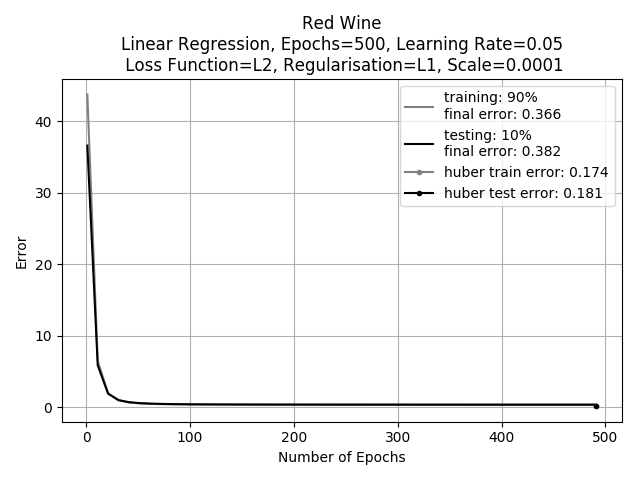
\includegraphics[width=0.9\linewidth]{img/l2_reg.png}
	\end{center}
	\caption{Red Wine - A good linear regression predictor with Ridge loss function and regularisation.}
	\label{fig:l2reg}
\end{figure}

\subsection{Neural Networks}
It was realised that ReLU for both hidden and output layers was by far the most effective activation function. This is because the ReLU function does not suffer from the vanishing gradient problem unlike functions such as tanh and sigmoid where the updating of weights can be prevented by a tiny gradient. 

It was also found that regularisation greatly improved the performance of neural net predictors. After running extensive tests with varying parameters and comparing the huber error of each of them, the best performing networks for both the white and red wine data sets can be seen below.

Regularisation is especially important for the neural nets as they have a tendency to over-fit. However the regularisation parameter, $\lambda$ has to be tuned correctly to avoid not fitting the data at all.

\begin{table}[]
	\begin{center}
	\begin{tabular}{l|l|}
		\cline{2-2}
		& Neural Network                                                    \\ \hline
		\multicolumn{1}{|l|}{No Reg} & 0.511                                                             \\ \hline
		\multicolumn{1}{|l|}{L1 Reg} & \begin{tabular}[c]{@{}l@{}}$\lambda = 0.001$\\ 0.504\end{tabular} \\ \hline
		\multicolumn{1}{|l|}{L2 Reg} & \begin{tabular}[c]{@{}l@{}}$\lambda = 0.1$\\ 0.513\end{tabular}   \\ \hline
	\end{tabular}
		\end{center}
	\caption{Comparison of \textbf{white wine} best neural network results after 500 epochs of training. Comparison error is the Huber Loss Function run after training.}
	\label{tab:nncomp}
\end{table}

\begin{table}[]
	\begin{center}
		\begin{tabular}{l|l|}
			\cline{2-2}
			& Neural Network                                                    \\ \hline
			\multicolumn{1}{|l|}{No Reg} & 0.447                                                             \\ \hline
			\multicolumn{1}{|l|}{L1 Reg} & \begin{tabular}[c]{@{}l@{}}$\lambda = 0.001$\\ 0.446\end{tabular} \\ \hline
			\multicolumn{1}{|l|}{L2 Reg} & \begin{tabular}[c]{@{}l@{}}$\lambda = 0.1$\\ 0.430\end{tabular}   \\ \hline
		\end{tabular}
	\end{center}
	\caption{Comparison of \textbf{red wine} best neural network results after 500 epochs of training. Comparison error is the Huber Loss Function run after training.}
	\label{tab:nncomp}
\end{table}


\subsection{Support Vector Machine Regression}
The linear support vector regression approach had quite similar results to basic linear regression with LASSO or Ridge loss functions, as can be seen in Tab \ref{tab:whiteresults} and Tab \ref{tab:redresults}, although the test error appeared to be more consistent. It was also found that having a large regularisation for SVR worsened the predictors performance as the data was greatly under-fitting.

Linear SVM Regression also was computationally expensive taking the longest time to run of all method implemented.

\section{Conclusion}
Models were trained and tested on a large dataset of both white and red wines. The task was to obtain a regression predictor with small test error. Multiple basic and advanced algorithms were implemented and tested, resulting in the conclusion that neural network models over-fit the data and require regularisation, however even with this do not compete with linear methods less prone to over-fitting. 

It was observed that test error was higher than training error for most cases.

Linear regression methods, LASSO, Ridge, SVR and Huber had a similar success rate, SVR appeared to be very consistent although the lowest error value is for a Ridge loss function.

It was found that the test error on the red wine data set was consistently less than the white, this is due to the data being highly concentrated in the former, making the prediction task easier.

{\small
	\bibliographystyle{ieee}
	\bibliography{egbib}
}


\section{Appendix}

\begin{figure}[h]
	\begin{center}
		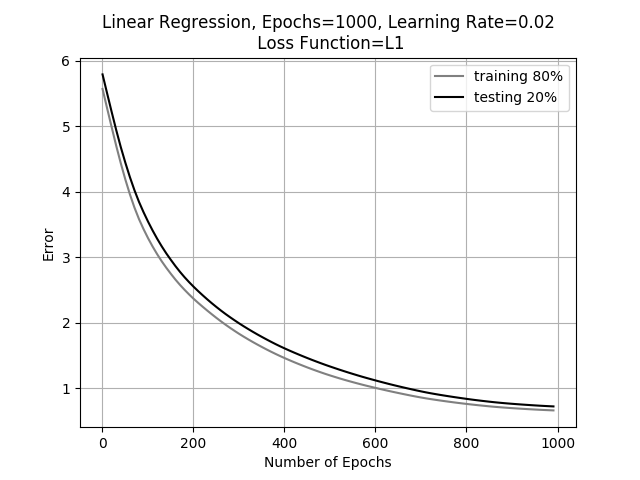
\includegraphics[width=0.9\linewidth]{img/l1loss.png}
	\end{center}
	\caption{Loss Function = LASSO, Training Error = 0.321, Testing Error = 0.373}
	\label{fig:l1loss}
\end{figure}

\begin{figure}[h]
	\begin{center}
		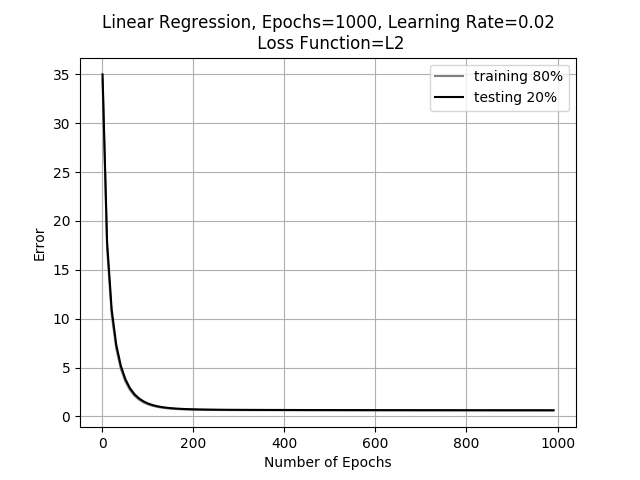
\includegraphics[width=0.9\linewidth]{img/l2loss.png}
	\end{center}
	\caption{Loss Function = Ridge, Training Error = 0.271, Testing Error = 0.276}
	\label{fig:l2loss}
\end{figure}

\begin{figure}[h]
	\begin{center}
		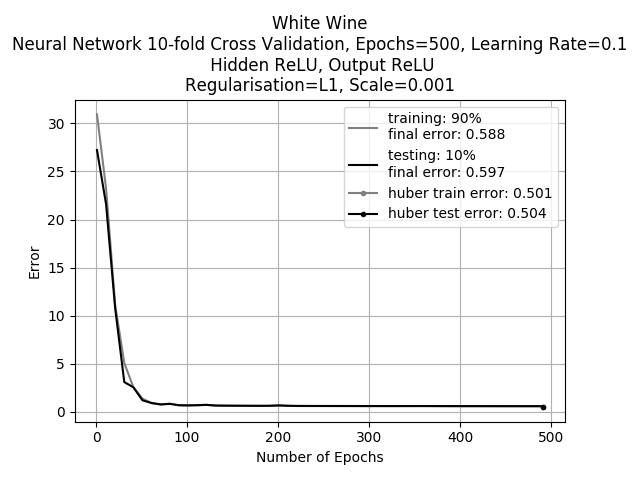
\includegraphics[width=0.9\linewidth]{img/best_white_nn.png}
	\end{center}
	\caption{Best Neural Network White Wine predictor.}
	\label{fig:wwbest}
\end{figure}

\begin{figure}[h]
	\begin{center}
		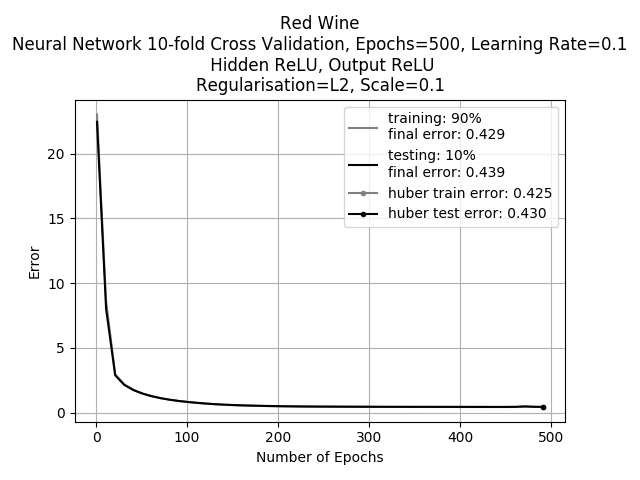
\includegraphics[width=0.9\linewidth]{img/best_red_nn.png}
	\end{center}
	\caption{Best Neural Network Red Wine predictor}
	\label{fig:rwbest}
\end{figure}

\end{document}
